\section{Introduction to Neural Networks}

Neural Networks are a type of a machine learning model inspired by activities in human brain.
A neural network comprises of `neurons`, which are considered as the building blocks.
A neuron in a neural network is implemented as weighted sum of its input, which is then passed through a non-linear function. This non-linear function is often denoted as an activation function and most commonly is a sigmoid or a rectified linear function.

Let $W$ be weights and $x$ denote the inputs. Let $g$ be the activation function, then a single neuron is represented as - 


\begin{figure}[H]
   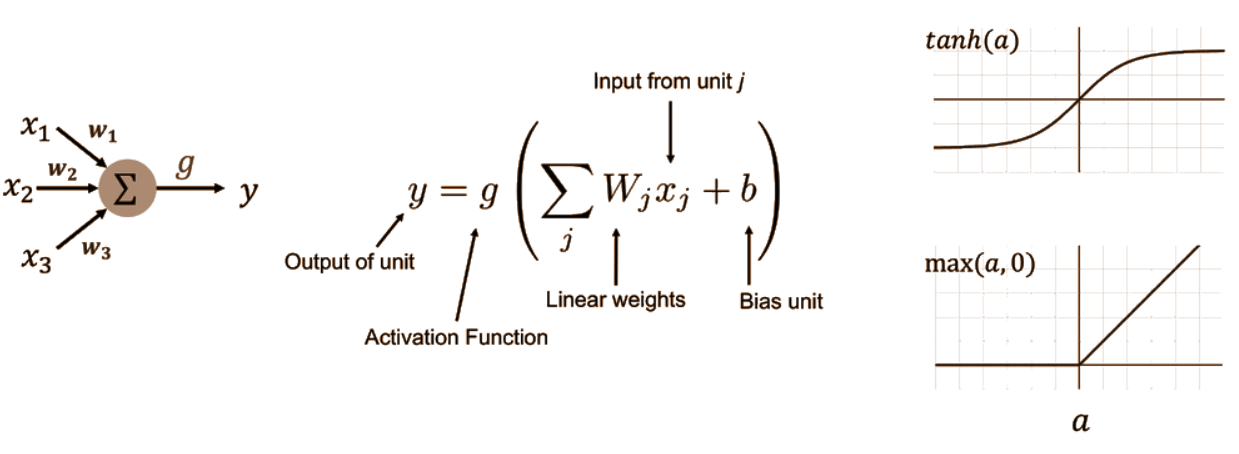
\includegraphics[width=1\linewidth, scale=0.9]{figures/intro/neuron.png}
   \caption[Artificial Neuron]{Artificial Neuron and common activation functions}
    \label{fig:neuron}
\end{figure}


When multiple of neurons are connected in a layer to all the inputs and the output of these neurons are used as input to another set of neurons, then the structure is called as Neural Network. This is shown in the figure ~\ref{fig:ann}


\begin{figure}[H]
	\centering
   \includegraphics[scale=0.66]{figures/intro/neural_network_start.bmp}
   \caption[Artificial Neuron]{Artificial Neuron and common activation functions}
   \label{fig:ann}
\end{figure}

\subsection{Learning}

Learning of Neural Networks is done in three steps --

\begin{enumerate}
	\item Forward pass
	\item Backward pass
	\item Weight upate
\end{enumerate}

During the forward pass the outputs are computed by multiplying the weights $w$ with the inputs (x). Let $w \times x$ be denoted as $e$ and the activation function be denoted as $f$, then output of a layer $f(e)$ would be $f_1(w_1 \times x_1 + w_2 \times x_2)$. 
If we consider the network shown in figure ~\ref{fig:ann}, then a single forward pass would be as depicted in the figure ~\ref{forward}.

\begin{figure}[H]
	\centering
   \includegraphics[scale=0.66]{figures/intro/forward.bmp}
   \caption[Forward pass]{Computation of a forward pass in a neural network}
   \label{fig:ann}
\end{figure}

\section{Introduction to Convolutional Neural Networks}